% !TeX spellcheck = cs_CZ

\documentclass[a4paper]{article}
\usepackage[english]{babel}
\usepackage[utf8x]{inputenc}
\usepackage[T1]{fontenc}
\usepackage{listings}
\usepackage[a4paper,margin=2cm]{geometry}
\usepackage{amsmath}
\usepackage{graphicx}
\usepackage[normalem]{ulem}
\usepackage[colorinlistoftodos]{todonotes}
\usepackage[colorlinks=true, allcolors=blue]{hyperref}
\usepackage{wasysym} % smileys
\usepackage{fancyhdr}
\setlength\parindent{0pt} % indent

% my commands:
\newcommand{\n}{\newline}
\newcommand{\tab}{\hspace{1cm}}

\def\repl#1#2{\textcolor{red}{\sout{#1}}\textcolor{blue}{#2}}
\def\XXX#1{\textcolor{red}{XXX #1}}

\begin{document}

\title{Ptakopět \\ \large Překlad tam a kontrolně zpět }
\author{Vilém Zouhar, Ondřej Bojar \small{(advisor)}}
\date{December 2018 \\ Rev. 4}
\maketitle 

\section{Overview}
Ptakopět (Překlad Tam A KOntrolně zPĚT) is an agile browser-agnostic plugin, which aims to help people translate to languages, where they are unable to verify the quality of the translation, by offering backward translation of the result. The issue at hand could be referred to as \textit{Outbound Translation}, which is a complement to \textit{Gisting}. Both in \textit{Gisting} and \textit{Outbound Translation}, a message is transferred between an author and a recipient the user has sufficient knowledge of only one of the languages. In \textit{Outbound Translation}, the user is responsible for creating correct messages, while in \textit{Gisting} the responsibility is to correctly interpret them. 

\subsection{The purpose of the project}
When translating to foreign languages users cooperate with machine translation tools to produce the best result. Many users use machine translation to verify their own translation, or can at least affirm, that the machine translation is valid. Translation systems are, however, not perfect and despite their great power, they tend to perform poorly on unseen phenomena (unknown words, unexpected word order, etc.). Users translating to languages, which they don't master enough to validate the translation could use Ptakopět to verify (and assure them), that the machine translation output is valid. Due to the fact that many encounters with foreign languages happen on the Internet, Ptakopět is developed as a browser extension.

\subsection{Other solutions}
Backward translation is only one of the solutions to \textit{Outbound Translation}. One of the possible solutions could include more autonomous systems, that would require less effort on the user side. This could be done with text highlighting, multiple translations or numeric responses (confidence intervals or just single number describing the system's certainty). Backward translation relies heavily on the ability of the user to assess the differences between texts.

\subsection{The scope}
Ptakopět aims to provide a backward translation interface to already existing translation engines. It does not do the translation itself in any way. Existing translation backends are provided by the Charles University, namely by Martin Popel and other associates. The interface is provided in a form of browser-agnostic plugin, that can also be hardwired to website as a plain script.

\pagebreak

\section{User interface}
\subsection{Usage}
Ptakopět runs as a small plugin located, if active, in top left or right corner. The intended workflow is to write text to the top textarea and validate against the backward translation in the bottom one. During this process, the translated text appears in the selected area on the web page. Active target input element is changed every time a possible element (all textareas and text inputs) gets focus.

\vspace{0.2cm}
\begin{figure}[h]
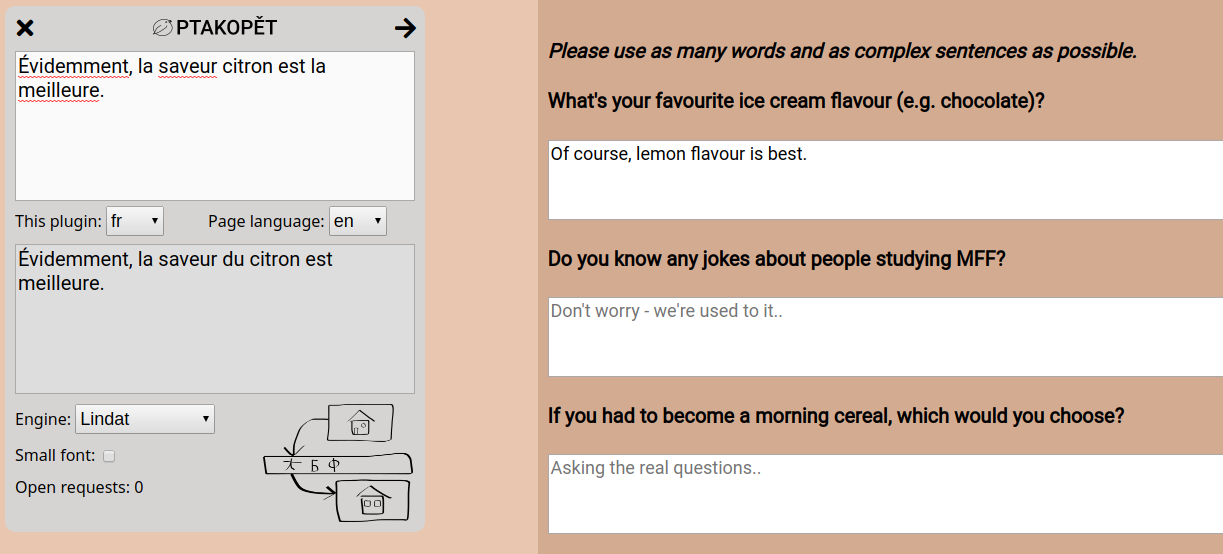
\includegraphics[width=\textwidth]{screenshot_3}
\caption{Ptakopět helps an French speaking user with filling in an English form}
\label{fig:screenshot_3}
\end{figure}
\vspace{0.2cm}

As seen in Figure \ref{fig:screenshot_3}, the user selected the first web page input element, hence making it active to Ptakopět and wrote a text in their native language (French) to the first Ptakopět input. The backward translation removed a definite article for an uncountable noun, otherwise the sentence matches the original.

The English translation of the input sentence appeared in the target textarea, as expected.

Should the user now edit the text in English, translation would appear in the bottom Ptakopět textarea. Writing into the top Ptakopět input field would overwrite the manual changes, as hinted in the bottom right diagram in the Ptakopět window in Figure \ref{fig:screenshot_3}.

\subsection{Activation, miscellaneous}
\begin{figure}[h]
\centering
\begin{minipage}{.5\textwidth}
  \centering
  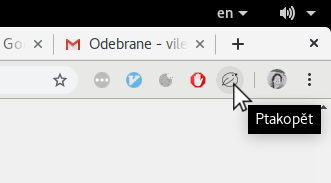
\includegraphics[width=0.9\textwidth]{screenshot_5}
  \caption{Ptakopět can be launched from toolbar}
  \label{fig:screenshot_5}
\end{minipage}%
\begin{minipage}{.5\textwidth}
  \centering
  \vspace{1.5cm}
  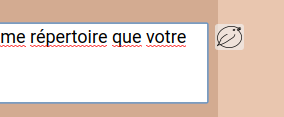
\includegraphics[width=0.9\textwidth]{screenshot_6}
  \caption{An icon for input activation appears next to possible text elements}
  \label{fig:screenshot_6}
\end{minipage}
\end{figure}
\vspace{0.3cm}

Ptakopět can be invoked in multiple ways: by clicking the toolbar button, as shown in Figure \ref{fig:screenshot_5}, by launching it from the context menu (right mouse button) or by clicking an icon, that appears next to all web page input elements. The last two methods also set the active input to the current input element.

\pagebreak

\begin{figure}[h]
\centering
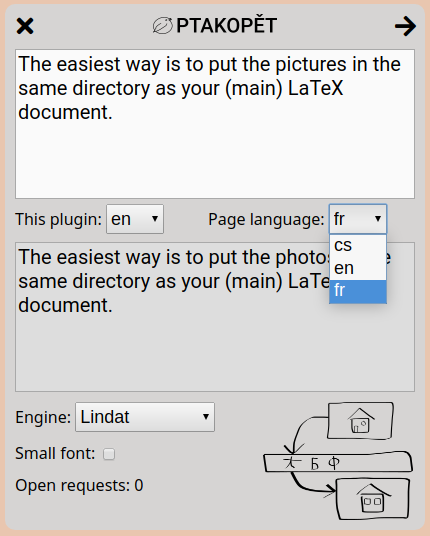
\includegraphics[width=0.4\textwidth]{screenshot_4}
\caption{Ptakopět plugin user interface}
\label{fig:screenshot_4}
\end{figure}
\vspace{0.3cm}

Source and target languages and backend engines can be swapped by the \textit{select} element, as shown in Figure \ref{fig:screenshot_4}. As of version 1.0.5, CS-EN and EN-FR language pairs are available for the Transformer Lindat backend \cite{transformer} and CS-EN, EN-ES, EN-DE, EN-FR for the Khresmoi service \cite{khresmoi}.\\
For convenience reasons, \textit{Small font} checkbox was added to allow work on larger texts.


\section{Implementation}
\subsection{Base structure}
The plugin itself is written in JavaScript, but injects HTML, CSS and jQuery framework into the web page. Making the plugin agnostic to whether it is run as a background script (browser plugin) or as an user script (included in web page) posed a substantial obstacle. Resulting implementation works, but is unfortunately affected by web styling. Eg.  website CSS can define the looks of the plugin, which is not intended and can result in usable, but not aesthetically pleasing design.
\subsection{Text inputs}
Ptakopět tries to capture all input events to \textit{textareas} and \textit{inputs}. This is a very robust approach, but about a half of the websites (as of 2018) use custom input elements (to provide styling and extra functionality). As a result, these elements can not be supported by Ptakopět. This is obviously a radical usability issue, but we didn't find any universal solution to this problem.
\subsection{Translation requests}
Text events are processed and forwarded to translation engine using AJAX requests. This could eventually pose a threat to these backends should the plugin be used by many people simultaneously. The engines would be glutted by requests, as every keypress invokes one or two translations. They are indistinguishable from legit requests, as the plugin works user-side. This could be solved by a standard approach of postponing requests to some interval of no key press (\textit{ptakopet\_arch.js:89}).
\subsection{GitHub repository structure}
The code itself is located in the \textit{src/} directory. The \textit{manifest.json} file is obligatory for all plugin versions. When Ptakopět is run as a background script (browser plugin), then \textit{ptakopet\_background\_bootstrap.js} is executed, which adds listeners to context menu and icons. Then \textit{ptakopet\_init.js} is run as a user script and from this point on, it is identical to having the script run from the web page. Due to asynchronous loading, the startup functions are called in \textit{ptakopet\_init\_user.js}. Generally, \textit{ptakopet\_init.js} handles visual elements (eg. displaying \textit{floater.html}, CSS etc.), while \textit{ptakopet\_translator.js} takes care of the translation flow. Ptakopět was designed to support fast addition of new translator backends or supported languages. Each translation object in Ptakopět manages it's own AJAX requests in a standardized form.

\section{Deployment}
\subsection{Standalone instalation}
This plugin can be also hardwired into a web page (mostly for presentation purposes). It is sufficient to download all source files (the \textit{src/} directory on GitHub) to some publicly available server foldre and add this line to your target HTML file: \begin{lstlisting}
<script id='ptakopet_init' src='path/to/ptakopet/js/ptakopet_init.js'></script>
\end{lstlisting}
All web pages containing this line of HTML will have the plugin activated. If a user has already Ptakopět installed, the server local version is used.

\subsection{Browser plugins}
Basic demonstration and info about Ptakopět online publication is located at \href{http://ptakopet.vilda.net}{ptakopet.vilda.net}. Ptakopět was also presented at MFF Open Days (November 2018). The presentation page is located at \href{https://vilda.net/s/dod\_ptakopet}{vilda.net/s/dod\_ptakopet}. The plugin itself is distributed as a \href{https://chrome.google.com/webstore/detail/ptakop\%C4\%9Bt/hgjlgmhmcmcmjiclegnipnaeejpibjmn}{Chrome} and \href{https://addons.mozilla.org/en-US/firefox/addon/ptakop\%C4\%9Bt/}{Firefox} extension. The plugin was also submitted to the Opera addon store, but still hasn't been reviewed.
Source code is published at a GitHub repository:\\ \href{https://github.com/zouharvi/ptakopet}{github.com/zouharvi/ptakopet}, the license is not yet decided, but feedback and code contributions are welcome.

\section{Future work}
Possible extensions could also include a full fledged web interface similar to that of Google Translate (one page). This could result in better user interface and overall clarity. Since Ptakopět is somewhat limited to backend capabilities, their extension is also desired (more language pairs, more information about translation confidence, etc.).

\section{Conclusion}
The first version of Ptakopět met all imposed usability criteria and didn't exceed the expected amount of work required.


\vspace*{\fill}

\begin{thebibliography}{1}
\bibitem{transformer}
  Martin Popel, Dušan Variš, Ondřej Košarko,
  Translation neural net model, build on top of Tensor2Tensor,
  ÚFAL, Lindat Clarin,
  17th December 2018
  \href{https://lindat.mff.cuni.cz/services/transformer/}{https://lindat.mff.cuni.cz/services/transformer/}
\bibitem{khresmoi}
  Ondřej Bojar,
  Medical information analysis and retrieval,
  ÚFAL,
  17th December 2018
  \href{https://ufallab.ms.mff.cuni.cz/~bojar/mt/khresmoi.php}{https://ufallab.ms.mff.cuni.cz/~bojar/mt/khresmoi.php}
\end{thebibliography}

\end{document}